\documentclass[10pt,a4paper]{article}
\usepackage[utf8]{inputenc}
\usepackage[english]{babel}
\usepackage{amsmath}
\usepackage{amsfonts}
\usepackage{amssymb}
\usepackage{graphicx}
%\usepackage{hyperref}
\usepackage[affil-it]{authblk}
\usepackage[left=2cm,right=2cm,top=2cm,bottom=2cm]{geometry}


\title{Semi-Lagrangian Exponential Integrator}
\author{P. S. Peixoto\thanks{pedrosp@ime.usp.br}\hspace{0.3cm} et al.}
\affil{College of Engineering, Mathematics and Physical Sciences - University of Exeter \\ Instituto de Matem\'atica e Estat\'\i stica - Universidade de S\~ao Paulo
}


\begin{document}
\maketitle

\section{Introduction}

Purpose: show a possible method to solve the nonlinear SWE with a semi-Lagrangian exponential integrator.

\section{Shallow Water Equations}
Consider the shallow water equations for a planar domain written as

\begin{eqnarray}
u_{t}+uu_{x}+vu_{y} &=&  fv -g\eta_x,\\
v_{t}+uv_{x}+vv_{y} &=& -fu- g\eta_y, \\
\eta_{t}+u\eta_{x}+v\eta_{y}&=&-\bar{\eta}( u_x +v_y) -\eta (u_{x}+ v_{y}), 
\end{eqnarray}
where the total fluid depth $h$ was decomposed into $h=\eta+\bar{\eta}$, where $\bar{\eta}$ is a constant mean fluid depth and $\eta$ is the perturbation. The velocities are given by $\vec{v}=(u,v)$ and the gravity $g$ is assumed constant. The Coriolis parameter $f$ is a function of $y$. 

Let the variables to be in a Lagrangian reference frame, $\vec{v}=\vec{v}(t,\vec{r}(t))$ and $\eta=\eta(t,\vec{r}(t))$, where $\vec{r}(t)=(x(t), y(t))$. Then we have for $\eta$ (and analogously for $u$ and $v$) that the total derivative is given as
\begin{equation}
\frac{d\eta}{dt}=\frac{\partial \eta}{\partial t}+\nabla \eta \cdot \vec{v} =  
\frac{\partial \eta}{\partial t} + u \frac{\partial \eta}{\partial x}+v\frac{\partial \eta}{\partial y},
\end{equation}
where we have used that $\vec{r}^{\,\prime}(t)=(x'(t), y'(t))=\vec{v}$. 
Considering the total derivatives given along flow trajectories, we will call $\gamma$ the parametrized trajectory curves in $(t, x, y)$ space, 
\begin{equation}
\gamma(s)=(s, x(s), y(s)).
\end{equation}
%For the line integrals we will require
%\begin{equation}
%\gamma'(s)=(1, x'(s), y'(s))=(1, u(s), v(s)),
%\end{equation}
%where we used that the velocities may be obtained from the derivatives of the position with time, $u(s)=x'(s)$ and $v(s)=y'(s)$. We also have that
%\begin{equation}
%\|\gamma'(s)\|=\sqrt{1 + u^2(s)+ v^2(s)}.
%\end{equation}
%Thus, the integral along a trajectory between two time steps will have the property that
%\begin{equation}
%\int_{t_n}^{t_{n+1}} d\gamma =\int_{t_n}^{t_{n+1}}\|\gamma'(s)\| ds= \int_{t_n}^{t_{n+1}}\sqrt{1 + u^2(s)+ v^2(s)} \, ds .
%\end{equation}
So the total derivative can be written as
\begin{equation}
\frac{d}{dt}= \gamma'(t) \cdot \left(\frac{\partial }{\partial t}, \frac{\partial }{\partial x},\frac{\partial }{\partial y} \right),
\end{equation}
with
\begin{equation}
\gamma'(s)=(1, x'(s), y'(s))=(1, u(s), v(s)).
\end{equation}


Also, we may express the linear wave operator as a matrix operator given by
\begin{equation}
L=
\left(\begin{array}{ccc}
  0 & f & -g\partial_{x}\\
 -f & 0 & -g\partial_{y}\\
 -\bar{\eta} \partial_{x}& -\bar{\eta} \partial_{x} & 0  
\end{array}\right).
\end{equation}


 This allows the shallow water equations to be written as
 \begin{equation}
\frac{dU}{dt}=LU+N(U), 
 \end{equation}
 where 
 \begin{equation}
 U=\left(\begin{array}{c}
  u\\
 v\\
 \eta  
\end{array}\right),
 \end{equation}
 
 \begin{equation}
 N(U)=\left(\begin{array}{c}
  0\\
 0\\
 -\eta \nabla\cdot \vec{v}  
\end{array}\right).
 \end{equation} 


\section{General semi-Lagrangian formulation}

For a review and details about semi-Lagrangian methods, please see \cite{Staniforth1991} and \cite{Durran2010}. 

\subsection{Trajectory calculations}

To calculate the trajectories one needs to solve the following ODE problem for $\vec{r}(t)=(x(t), y(t))$,
\begin{equation}
\frac{d \vec{r}(t)}{dt} = \vec{v}(t, \vec{r}(t)),
\end{equation}
with 
\begin{equation}
\vec{r}(t_0) = (x(t_0), y(t_0)).
\end{equation}

This can be done through many of existing techniques (see \cite{Staniforth1991} and \cite{Durran2010}).  We will discuss two possibilities in this section.

\subsubsection*{Basic 2-time-level}

A simple approach uses fixed point iterations using the method of \cite{Robert1981}, but following a two-time level method as in \cite{McDonald1987}. Integrating from time $t_n$ to time $t_{n+1}$ we have that
\begin{equation}
\vec{r}(t_{n+1})-\vec{r}(t_{n}) = \int_{t_n}^{t_{n+1}}\vec{v}(t, \vec{r}(t))dt.
\end{equation}
Numerically we can calculate departure points $\vec{r}_d=\vec{r}(t_{n})$ using the arrival grid points $\vec{r}_a=\vec{r}(t_{n+1})$ and the trajectory midpoint $\vec{r}_m=\vec{r}(t_{n+1/2})$ as
\begin{equation}
\vec{r}_a-\vec{r}_d = \vec{v}(t_{n+1/2}, \vec{r}_m) \Delta t,
\end{equation}
and
\begin{equation}
\vec{r}_a-\vec{r}_m = \vec{v}(t_{n+1/2}, \vec{r}_m) \frac{\Delta t}{2},
\end{equation}
and solving iteratively the equation for the midpoints with
\begin{equation}
\vec{r}^{\,k+1}_m = \vec{r}_a-\vec{v}(t_{n+1/2}, \vec{r}^{\,k}_m) \frac{\Delta t}{2},
\end{equation}
with $\vec{r}^{\,0}_m=\vec{r}_a$. Two or three iterations are usually enough to obtain a good estimate for the midpoint. The departure point can then be estimated by 
\begin{equation}
\vec{r}_d=\vec{r}_m - \vec{v}(t_{n+1/2}, \vec{r}_m) \frac{\Delta t}{2}=2\vec{r}_m-\vec{r}_a.
\end{equation}
Extrapolation methods are required to obtain the velocity at the trajectory midpoints, this may be obtained as
\begin{equation}
\vec{v}(t_{n+1/2}, \vec{r}^{\,k}_m)=\left(\frac{3}{2}\vec{v}(t_{n})-\frac{1}{2}\vec{v}(t_{n-1}) \right)_m,
\label{eq:extrap_simp}
\end{equation}
where the sub-index $_m$ indicates that once the extrapolation is done, it is then interpolated to the trajectory midpoints $\vec{r}^{\,k}_m$.

%It is common that only the arrival and departure point informations are used, to reduce the amount of interpolations, so the interpolation to midpoints is substituted by averages of the values at the arrival and departure points, to yield,
%\begin{equation}
%\vec{v}(t_{n+1/2}, \vec{r}^{\,k}_m)=\frac{1}{2}\left( \frac{3}{2}\vec{v}(t_{n})-\frac{1}{2}\vec{v}(t_{n-1})\right)  + \frac{1}{2}\left( \frac{3}%{2}\vec{v}(t_{n})-\frac{1}{2}\vec{v}(t_{n-1}) \right)_*.
%\end{equation}

\subsubsection*{Stable Extrapolation Two-Time-Level Scheme}
\label{sec:stable}
The extrapolation scheme shown above tends to be unstable for large time steps for the nonlinear shallow water equations \cite{Durran2010}. An alternative is the Stable Extrapolation Two-Time-Level Scheme (SETTLS) of \cite{Hortal2002}, used in the ECMWF global model IFS.

This approach uses as extrapolation method along the trajectories, for any given function $\phi$,
\begin{equation}
\phi(t_{n+1/2}, \vec{r}_m)=\frac{1}{2}\left(2\phi(t_{n}, \vec{r}_d)-\phi(t_{n-1}, \vec{r}_d) + \phi(t_{n}, \vec{r}_a)\right).
\end{equation}
So the velocity at the midpoints may be approximated as
\begin{equation}
\vec{v}(t_{n+1/2}, \vec{r}^{}_m)=\frac{1}{2} \left(2\vec{v}(t_{n}, \vec{r}_d)-\vec{v}(t_{n-1}, \vec{r}_d) + \vec{v}(t_{n}, \vec{r}_a) \right).
\end{equation}

The departure point can be obtained through an iterative procedure as before with, 
\begin{equation}
\vec{r}^{\,k+1}_d = \vec{r}_a- \frac{\Delta t}{2} \left(2\vec{v}(t_{n}, \vec{r}_d^{\,k})-\vec{v}(t_{n-1}, \vec{r}_d^{\,k}) + \vec{v}(t_{n}, \vec{r}_a) \right),
\end{equation}
with first guess given using $\vec{r}^{\,0}_d=\vec{r}_a$.

%\begin{equation}
%\vec{r}^{1}_d = \vec{r}_a- \frac{\Delta t}{2} \left(3\vec{v}(t_{n}, \vec{r}_a)-\vec{v}(t_{n-1}, \vec{r}_a)  \right),
%\end{equation}
The fields to be calculated at the departure points, such as $\vec{v}(t_{n}, \vec{r}_d^{\,k})$, will be done first calculating $\vec{v}(t_{n})$ at the usual grid points, and then this will be interpolated to the departure points $\vec{r}_d^{\,k}$. We will denote this interpolation to departure points with a $*$, to give the following formulas
\begin{equation}
\vec{r}^{\,k+1}_d = \vec{r}_a- \frac{\Delta t}{2} \vec{v}(t_{n} ) - \frac{\Delta t}{2} \left(2\vec{v}(t_{n})-\vec{v}(t_{n-1})\right)_*  .
\end{equation}

A second order interpolation for the velocity is usually enough to ensure an overall second order accurate semi-Lagrangian method \cite{Peixoto2014}.


\subsection{Integrating factor}

Let $I$ be defined as the solution to the problem 
\begin{equation}
\frac{dI}{dt}=-IL,
 \end{equation}
 subject to
\begin{equation}
I(t_n)=\text{Id},
 \end{equation}
 where $\text{Id}$ is the identity matrix.
 
 
Considering the integral as being element-wise in $L$, it is easily verified that the problem has solutions of the form
\begin{equation}
I=e^{-\int_{t_n}^t L(\gamma(s))\, ds},
\end{equation} 
where $\gamma(s)$ is the trajectory curve  parametrization related to $d/dt$. This $I$ will be denoted as the integrating factor.

%since
%\begin{equation}
%\frac{d }{dt} \int_{t_n}^{t} L_{ij}(\gamma(s))ds =
%L_{ij}(\gamma(t)),
%\end{equation}
%for $L_{ij}$, $i,j=1,2,3$ elements of $L$, 

%where the primitive is considered along trajectories ($\gamma$) and are such that
%\begin{equation}
%\frac{D }{Dt}\left(\int L d\gamma \right)=L.
%\end{equation} 

%
%Since $L=L(t,x(t), y(t))=L(\gamma(t))$, considering the integral as being element-wise in $L$, we have for an element $L_{ij}$, $i,j=1,2,3$,
%\begin{equation}
%\frac{d }{dt} \int_{t_0}^{t} L_{ij}(\gamma(s))ds =
%L_{ij}(\gamma(t)),
%\end{equation}
%and thus,  
%\begin{eqnarray}
%\frac{dI}{dt}&=&\frac{d}{dt} \left(e^{-\int_{t_0}^t L(s, x(s), y(s))\, ds} \right) \\
%& =& -e^{-\int_{t_0}^t L(s, x(s), y(s))\, ds} \frac{d}{dt} \left(\int_{t_0}^t L(s, x(s), y(s))\, ds \right) \\
%&=& -e^{-\int_{t_0}^t L(s, x(s), y(s))\, ds} L(t, x(t), y(t))\\
%&=&-IL.
%\end{eqnarray}

We will also need the inverse of the integrating factor, which we will call $J$,  defined as
\begin{equation}
J=e^{\int_{t_n}^t L(\gamma(s))\, ds},
\end{equation} 
for which one readily sees that $IJ$ is the identity matrix.

\subsection{Semi-Lagrangian method}
Using the above defined integrating factor $I$, we may write the shallow water equations as
\begin{equation}
I\frac{dU}{dt}=ILU+IN(U), 
\end{equation}
which, using the definition of the integrating factor and the properties of the derivative, can be transformed to 
\begin{equation}
I\frac{dU}{dt}=-\frac{dI}{dt}U+IN(U), 
\end{equation}
\begin{equation}
\frac{d(IU)}{dt}=I N(U).
\end{equation}

To derive the semi-Lagrangian formulation we assume that the solution is known at grid points at a time step $t_n$ and wish to calculate the solution at time $t_{n+1}$. Integrating the above equation along trajectories gives us 
\begin{equation}
(IU)^{n+1}-(IU)^{n}_{*}=\int_{t_n}^{t_{n+1}} I(t, \vec{r}(t))\, N(U(t, \vec{r}(t)))\, dt,
\end{equation}
where $*$ indicates that this value should be at trajectories departure points and the integral is along trajectories. The integrating factor $I$ is the identity at the departure points, so the resulting method for calculation of the new values at grid points can be calculated as
\begin{equation}
U^{n+1}=J^{n+1}(  U)^{n}_{*}+J^{n+1}\int_{t_n}^{t_{n+1}} \, I(t, \vec{r}(t))\, N(U(t, \vec{r}(t)))\,dt .
\end{equation}
We see that this is very similar to the usual exponential integrator equation in Eulerian forms.

To solve this equation, the trajectories and departure points may be calculated with any of the several existing flavours. We will discuss possible approximation for the right hand side of the equation in what follows.

\section{Non-divergent flow case}

Here we will analyse the case when the flow is non-divergent, therefore, $N(U)=0$, and we need to solve only

\begin{equation}
\frac{dU}{dt}=L U,
\label{eq:swe}
\end{equation}
where all the non-linearities are in the material derivative.


\subsection{On a f-plane} 

Consider the shallow water equations given for a bi-periodic plane with $f$ constant. In this case $L$ is constant along the trajectories, so
\begin{equation}
U^{n+1}=J^{n+1}U^{n}_{*},
\end{equation}
with
\begin{equation}
 J^{n+1}=e^{L\Delta t}
\end{equation}
and the method may be written as
\begin{equation}
U^{n+1}=e^{L\Delta t}(U)^{n}_{*}.
\end{equation}

Since $e^{L\Delta t}$ is constant, we can allow ourselves to apply it as  
\begin{equation}
U^{n+1}=(e^{L\Delta t} U)^{n}_{*},
\end{equation}
which means that in practice we can first calculate 
$
e^{L\Delta t} U,
$
with any given matrix exponentiation method, and then interpolate this to quantity to the departure points.


\subsection{On a variable $f$ scenario}

We will now allow the Coriolis parameter $f$ to vary in the $y$ direction, for example as in the $\beta$-plane approximation $f=f_0+\beta y$ or, on the spherical case, $f=2\Omega \sin \theta$, where $\theta$ is the latitude, and $\Omega$ is the rotation rate of the Earth. In this case, $L$ is no longer constant along trajectories and the integrating factor needs to be approximated. 

\subsubsection{$f$ constant along trajectories}

Considering that the trajectories spam a small region in space for which the variation of $f$ is small, we may approximate the integrating factor considering the Coriolis parameter given for the trajectory midpoint. That is
\begin{equation}
J^{n+1}=e^{\int_{t_n}^{t_{n+1}}L(\gamma(t))dt}  \approx e^{L(\gamma(t_{n+1/2})) \int_{t_n}^{t_{n+1}}dt} = e^{L^{1/2}\Delta t},
\end{equation}
 where $L^{1/2}$ is the linear operator calculated at the trajectory midpoint $\vec{r}_m$. The resulting method is similar to the $f$-plane case,
\begin{equation}
U^{n+1}=(e^{L^{1/2}\Delta t} U)^{n}_{*}.
\end{equation}
 
The problem with this approach is that the exponential integrator will depend on the trajectory points, which can make it impractical with REXI, since these the midpoints are not necessarily grid points. 

If we consider a constant approximation of $L$ along trajectories, with reference values given for the time $t_n$, then 
\begin{equation}
J^{n+1}=e^{\int_{t_n}^{t_{n+1}}L(\gamma(t))dt} \approx e^{L(\gamma(t_n))\int_{t_n}^{t_{n+1}}dt} = e^{L \Delta t},
\end{equation}
then
\begin{equation}
U^{n+1}=(e^{L \Delta t} U)^{n}_{*}.
\end{equation}
where $e^{L \Delta t} U$ is the usual exponential integrator but considering the variations of $f$ given for the time $t_n$. 

The consequences of the latter approximation is that the Rossby waves might not be well represented if the time-step is too large.






\section{Full nonlinear case}

Considering the above method, where $L$ is constant along trajectories, then we may write the the method for the full non linear case as 
\begin{equation}
U^{n+1}=(e^{L \Delta t} U)^{n}_{*}+e^{L\Delta t}\int_{t_n}^{t_{n+1}} \, I(t, \vec{r}(t))\, N(U(t, \vec{r}(t)))\,dt.
\end{equation}

\subsection{Standard Exponential Integrator Scheme}
This can be worked out in several ways (like Cox and Mathews). A simple way is to consider a forward Euler method for the nonlinear part, as 
\begin{eqnarray*}
e^{L\Delta t}\int_{t_n}^{t_{n+1}} \, I(t, \vec{r}(t))\, N(U(t, \vec{r}(t)))\,dt &\approx & 
e^{L\Delta t} \left( \int_{t_n}^{t_{n+1}}  I(t, \vec{r}(t))\,dt \right) N(U(t_n))_*\\
&= & 
e^{L\Delta t} \left( \int_{t_n}^{t_{n+1}} \frac{d I(t, \vec{r}(t))}{dt}L^{-1}\,dt \right) N(U(t_n))_*\\
&\approx & 
e^{L\Delta t} \left(  I(t_{n+1}, \vec{r}(t_{n+1}))- I(t_{n}, \vec{r}(t_{n})) \right) L^{-1} N(U(t_n))_*\\
&= & 
e^{L\Delta t} \left( e^{-L\Delta t} - \text{Id} \right) L^{-1} N(U(t_n))_*\\
&= & 
 \left(   \text{Id} - e^{L\Delta t}\right) L^{-1} N(U(t_n))_*\\
&\approx & 
 \left(\left(   \text{Id} - e^{L\Delta t}\right) L^{-1} N(U(t_n))\right)_*,
\end{eqnarray*}
where we use that the $I$ is constant along trajectories (but might not be constant in the domain), resulting in 
\begin{equation}
U^{n+1}=(e^{L \Delta t} U)^{n}_{*}+\left(\left(   \text{Id} - e^{L\Delta t}\right) L^{-1} N(U)\right)^{n}_*.
\end{equation}
which can be calculated as
\begin{equation}
U^{n+1}=\left(e^{L \Delta t} U+\left(   \text{Id} - e^{L\Delta t}\right) L^{-1} N(U)\right)^{n}_*.
\end{equation}

The problem with using standard exponential integrator approaches, such as Cox and Mathews, is that they rely on the having $L^{-1}$, which, in the case of SWE, is not well defined in general, since the kernel is non trivial (it has all the geostrophic modes).


\subsection{Alternative scheme}

In semi-Lagrangian methods, it is common that the nonlinear terms are discretized as averages of the departure and arrival trajectory points given for the intermediate time $t_{n+1/2}$.

% This is equivalent to using the trapezoidal rule for the integral of the nonlinear part as
%\begin{equation}
%\int_{t_n}^{t_{n+1}} \, I(t, \vec{r}(t))\, N(U(t, \vec{r}(t)))\,dt \approx \frac{\Delta t}{2} \left[ I(t_{n+1}, \vec{r}_a)\, N(U(t_{n+1}, \vec{r}_a)+I(t_{n-1}, \vec{r}_d)\, N(U(t_{n-1}, \vec{r}_d))\right]
%\end{equation}

This leads to the following approach,
\begin{equation}
U^{n+1}=(e^{L \Delta t} U)^{n}_{*}+\frac{\Delta t}{2}e^{L\Delta t}\left[ I(t_{n+1/2}, \vec{r}_a)\, N(U(t_{n+1/2}, \vec{r}_a)+I(t_{n+1/2}, \vec{r}_d)\, N(U(t_{n+1/2}, \vec{r}_d))\right],
\end{equation}
which, using the assumption of constant $L$ along trajectories,
\begin{equation}
 I(t_{n+1/2}, \vec{r}(t))=e^{-L\Delta t/2},
\end{equation} 
may be simplified to
\begin{equation}
U^{n+1}=(e^{L \Delta t} U)^{n}_{*}+\frac{\Delta t}{2}e^{L\Delta t/2}\left[ N(U(t_{n+1/2}, \vec{r}_a)+ N(U(t_{n+1/2}, \vec{r}_d))\right],
\end{equation}
or
\begin{equation}
U^{n+1}=\left(e^{L \Delta t} U^n +\frac{\Delta t}{2}e^{L\Delta t/2}N(U)^{n+1/2}\right)_{*}+\frac{\Delta t}{2}e^{L\Delta t/2} N(U)^{n+1/2}.
\end{equation}

Since $N(U)$ is required at an intermediate time-step, this needs to be extrapolated from previous values of $N(U)$ given in time steps $n$ and $n-1$. Using the same extrapolation as in equation \eqref{eq:extrap_simp}, the resulting method is
\begin{equation}
U^{n+1}=\left[e^{L \Delta t} U^n +\frac{\Delta t}{2}e^{L\Delta t/2}\left(\frac{3}{2}N(U^n)-\frac{1}{2}N(U^{n-1})\right)\right]_{*}+\frac{\Delta t}{2}e^{L\Delta t/2} \left(\frac{3}{2}N(U^n)-\frac{1}{2}N(U^{n-1})\right).
\end{equation}

\subsection{Stable scheme}


As discussed in section \ref{sec:stable}, using standard extrapolation schemes may lead to an unstable scheme. An option is to use the SETTLS approach, which would give
\begin{equation}
U^{n+1}=(e^{L \Delta t} U)^{n}_{*}+\Delta t \, e^{L\Delta t/2}\left[  N(U(t_{n+1/2}, \vec{r}_m)\right],
\end{equation}
where 
\begin{equation}
 N(U(t_{n+1/2}, \vec{r}_m)) = 
\frac{1}{2}\left[2 N(U(t_{n}, \vec{r}_d))- N(U(t_{n-1}, \vec{r}_d))+  N(U(t_{n}, \vec{r}_a))\right],
\end{equation}
which may be calculated as
\begin{equation}
 N(U(t_{n+1/2}, \vec{r}_m)) = 
\frac{1}{2}\left[ 2 N(U(t_{n}))- N(U(t_{n-1}))\right]_* +  \frac{1}{2}\left[N(U(t_{n}))\right].
\end{equation}


The resulting method is 
\begin{equation}
U^{n+1}=\left[e^{L \Delta t} U^n+\Delta t\,e^{L\Delta t/2}\left( N(U^n)- \frac{1}{2}N(U^{n-1})\right) \right]_*+\frac{\Delta t}{2}e^{L\Delta t/2}N(U^n).
\end{equation}

To save on calculations, one may calculate
\begin{eqnarray}
V^n&=&e^{L \Delta t} U^n \\
W^n&=&e^{L \Delta t/2} N(U^n)
\end{eqnarray}
and then
\begin{equation}
U^{n+1}=\left[V^n+\Delta t\,W^n - \frac{\Delta t}{2}W^{n-1} \right]_*+\frac{\Delta t}{2}W^n.
\end{equation}

For the interpolation to departure points, a third order interpolation method is recommended to ensure overall second order accuracy of the semi-Lagrangian scheme \cite{Peixoto2014}.
%
%\subsection{Calculations of $e^{L\Delta t}N(U)$ }
%
%Since $N(U)=(0,0,\psi)$, it might be possible to simplify the calculation of $e^{L\Delta t}N(U)$ in REXI.

\section{Lagrangian treatment of Coriolis term}

The treatment of variable Coriolis term is complicated with the above approach for 2 reasons: First, it needs to be approximated along the trajectories, which could affect the Rossby waves, second, the exponential integrator has to deal with non constant coefficient solvers, which can be far more complicated and expensive.

For these reasons, here we will briefly describe the possibility of treating the Coriolis term in a Lagrangian fashion.

\subsection{Planar case}
We may write the momentum equations as

\begin{eqnarray}
\frac{du}{dt}&=&  f(y)v -g\eta_x,\\
\frac{dv}{dt} &=& -f(y)u- g\eta_y, 
\end{eqnarray}
or in vector notation,
\begin{equation}
\frac{d\vec{u}}{dt}+f(y)\vec{k}\times\vec{u}=-\nabla \eta, 
\end{equation}
where $\vec{u}=(u,v)$, and $\vec{k}=(0,0,1)$ is a vector normal to the plane. Now notice that 
\begin{equation}
\frac{d \vec{r}}{dt} = \vec{v},
\end{equation}
so we have that
\begin{equation}
\frac{d\vec{u}}{dt}+f(y)\vec{k}\times\frac{d \vec{r}}{dt}=-\nabla \eta, 
\end{equation}

If $f(y)=f$ constant (f-plane approximation), then
\begin{equation}
\frac{d\left( \vec{u} + f\vec{k}\times \vec{r}\right)}{dt}=-\nabla \eta, 
\label{eq:lag_coriolis_plan}
\end{equation}
which means that the Coriolis term can be solved together with the lagrangian advected quantity. 

If $f$ is to be assumed dependent on $y$, then the above equation \eqref{eq:lag_coriolis_plan} only makes sense considering the assumption that $f(y)$ is constant along trajectories. 

\subsection{Spherical case}

Although it is not possible to consider the variable $f$ case lagrangianly on a plane, this is different for the sphere. It is described in \cite{Temperton1997} how it is possible to treat the Coriolis term in a lagrangian way even in the variable $f$ condition. As a consequence, the exponential computational (REXI) would treat only the gravity waves, but not the Rossby ones.

We will briefly describe this case here (soon).

\section{Numerical results}


\subsection{Non-divergent flows}

Geostrophically balanced solution of the nonlinear equations.

\begin{eqnarray}
h&=&\cos\left( 2 \pi (x/L_x+y/L_y)\right)+ \bar{\eta}\\
u&=&\frac{2 g \pi}{f_0 L_y} \sin\left( 2 \pi (x/L_x+y/L_y)\right)\\
v&=&-\frac{2 \pi g}{f_0 L_x} \sin\left( 2 \pi (x/L_x+y/L_y)\right)
\end{eqnarray}

This test has trajectories given as straight lines, but these are not coinciding with the grid. Therefore, the departure point calculation is expected to be very accurate, and the errors associated with the semi-lagrangian are mainly related to interpolation errors of the field at the departure points. 

Since the flow is non-divergent, the non advective nonlinear term (divergence term of continuity equation) is assumed to be zero.

\begin{figure}
\centering
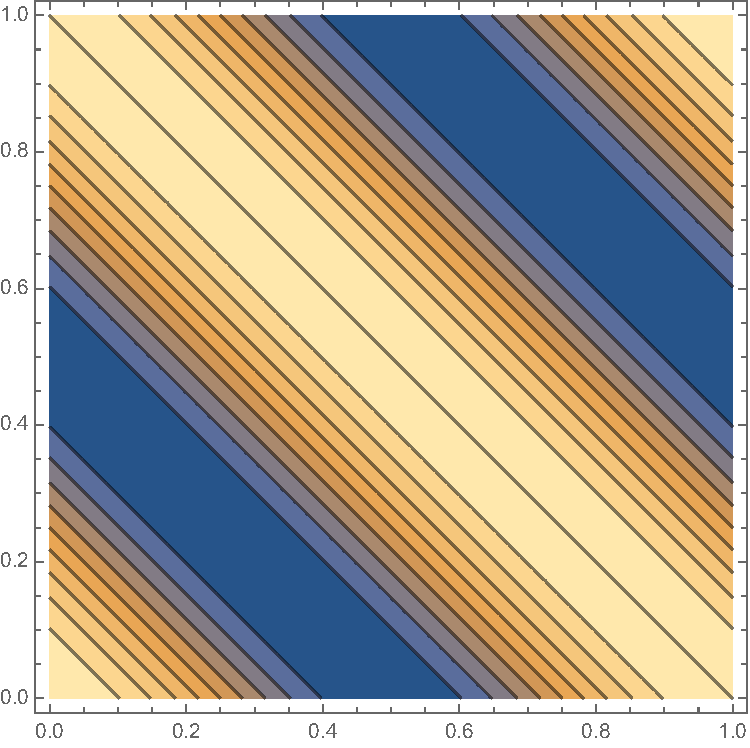
\includegraphics[scale=0.4]{geobalance_rotated_h.pdf} 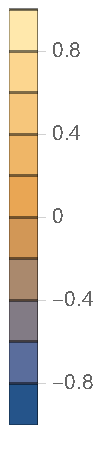
\includegraphics[scale=0.4]{geobalance_rotated_hscale.pdf} \hspace{1cm}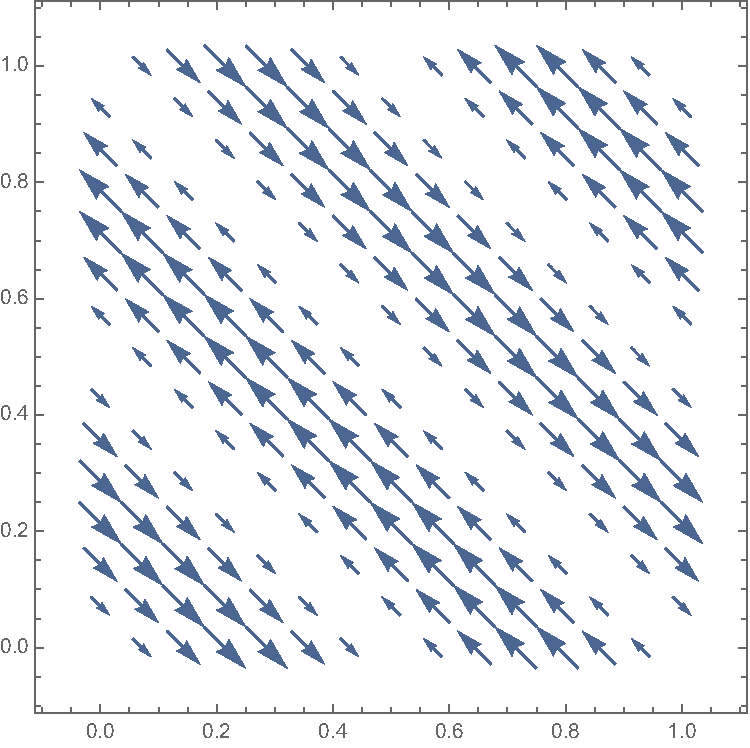
\includegraphics[scale=0.4]{geobalance_rotated_uv.pdf} 
\caption{Height and velocity fields for steady state rotated non-divergent flow}
\end{figure}

\subsection{Non-divergent Forced flow }
\begin{eqnarray}
h&=&\cos(2 \pi x/L_x)\sin(2\pi y /L_y) + \bar{\eta}\\
u&=&-\frac{2 g \pi}{f_0 L_y} \cos(2\pi x/L_x) \cos(2\pi y /L_y)\\
v&=& -\frac{2 \pi g}{f_0 L_x} \sin(2\pi x/L_x) \sin(2\pi y/L_y)\\
\end{eqnarray}
with forcings
\begin{eqnarray}
f_h&=&0\\
f_u&=&-\frac{\pi}{L_x}\left(\frac{2 \pi g}{f_0 L_y}\right)^2 \sin(4\pi x/L_x)\\
f_v&=& \frac{\pi}{L_y}\left(\frac{2 \pi g}{f_0 L_x}\right)^2 \sin(4\pi y/L_y)\\
\end{eqnarray}

\subsection{Divergent flows}


\section{Concluding remarks}





\appendix



\bibliographystyle{alpha}
\bibliography{bibliography}
% 
%where $U=(h, u, v)$ is the vector of unknowns containing the the velocity $\vec{v}=(u,v)$ and the fluid height perturbation ($h$), $L$ is the linear shallow water operator given by
%where $H_0$ is the mean water depth (assumed constant),  and the $D/Dt$ is the material (total) derivative given by
%\begin{equation}
%\frac{D}{Dt}=\frac{\partial }{\partial t}+\vec{v}\cdot \nabla.
%\end{equation} 
%  
%We will consider $U$ in its moving/Lagrangian framework, that is, $U(\vec{p}(t),t)$ depends on a position $\vec{p}(t)=(x(t),y(t))$ which varies with time.
%
%%Let $I$ be the an indefinite primitive of the linear exponential along an arbitrary trajectory,
%%\begin{equation}
%%I=\oint e^{sL}L \, ds,
%%\end{equation} 
%%such that 
%%\begin{equation}
%%\frac{D I}{Dt}=e^{tL}L.
%%\end{equation}
%
%If $L$ is independent of space, therefore constant along the trajectory (for example on a f-plane), then
%\begin{equation}
%\frac{De^{-tL}}{Dt}=-e^{tL} L ,
%\end{equation}
%which can be used to reduce \eqref{eq:swe} by multiplying it by $e^{-tL}$, 
%\begin{equation}
%e^{-tL}\frac{DU}{Dt}=e^{-tL} L U,
%\end{equation}
%which can be written as
%\begin{equation}
%e^{-tL}\frac{DU}{Dt}=-\frac{De^{-tL}}{Dt} U,
%\end{equation}
%and therefore
%\begin{equation}
%\frac{D (e^{-tL}U)}{Dt}=0,
%\end{equation}
%
%Now integrating between times $t_n$ and $t_n{n+1}$ along an arbitrary trajectory gives
%\begin{equation}
%(e^{-t_{n+1}L}U)^{n+1}=(e^{-t_nL}U)^{n}_{*},
%\end{equation}
%where the star ($*$) indicates that the value is given for the departure point of the trajectory. Since in the f-plane the exponential is invariant along trajectories, we may write it as
%\begin{equation}
%U^{n+1}=e^{t_{n+1}L}(e^{-t_nL}U)^{n}_{*},
%\end{equation}
%\begin{equation}
%U^{n+1}=(e^{\tau L}U)^{n}_{*},
%\end{equation}
%where $\tau=t_{n+1}-t_n$.
%
%\section{Numerical implementation}
%Given a state $U^n$ at time $t_n$, the first step is to propagate the exponential integrator, 
%\begin{equation}
%U_L^{n}=e^{\tau L}U^n.
%\end{equation}
%
%Now for all grid points, the back-trajectory should be estimated to obtain their respective departure points. Any two time level trajectory calculation can be used here (usually 3 iterations of the nonlinear equation . 
%
%
%his can be multiplied by $e^{-t_nL}$

\end{document}
